\subsection{Future Work} 

As seen in Figure~\ref{fig:sprint_4} there are several issues that were
not yet resolved. For future development these should be implemented for an
enhanced user experience.

\begin{figure}[H]
\centering
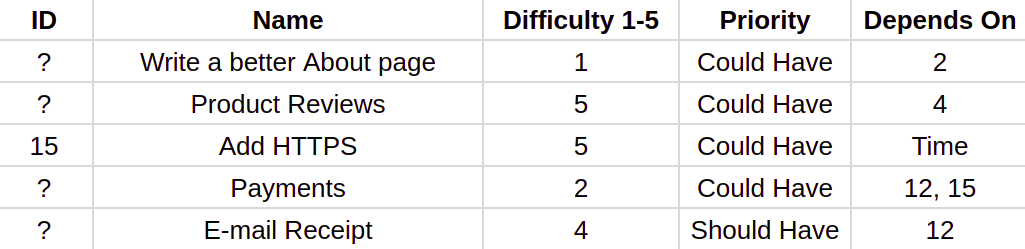
\includegraphics[width=\textwidth]{third_sprint/other.png}
\caption{\label{fig:sprint_4} Issues for future work}
\end{figure}

\subsubsection{About Page}\label{sec:about}

To update the About page was ignored since this project is more of a proof
of concept than a fully deployed web shop, but should be implemented before
actually starting a business to build trust with users.

\subsubsection{Transactions}\label{sec:transaction}

In the implementation shown in the last demo, there was no atomicity
constraints at the checkout of orders. This is something that would have to be
fixed if the service were ever to be used live. It would be a imple matter of
wrapping the transactions in the following \mintinline{python}{with}-statement
(See Figure~\ref{fig:transaction}).

\begin{figure}[H]
\centering
\begin{minted}{python}
from django.db import transaction
with transaction.atomic():
  # Any code here will be considered one transaction.
  pass
\end{minted}
\caption{\label{fig:transaction} How to wrap database interaction within
Django in order to ensure atomic transactions.}
\end{figure}


\subsubsection{Proper Order Handling}\label{sec:security}

The three last issues \textit{Add HTTPS, Payments, and E-mail Receipt}, would
be be critical for completing the last chapter of this web shop. Although these
implementations would require additional thought regarding managing tables
and the DBMS, the technologies are rather outside of the scope of this course.

Django has implementation guides for including HTTPS to the Django-App,
so that part should be rather easily implemented. Adding an automated email
service is also something that could be implemented via the Django-framework.
Payment systems on the other hand would require a dive into a completely
new technology-field. Given that this is not the objective of this course,
the chances of this being implemented are slim, it would nevertheless be
interesting and fun to implement such functionality.
